\documentclass{article}
\usepackage{graphicx}
\usepackage{amsmath}
\usepackage{hyperref}
\usepackage{ragged2e}
\usepackage{tikz}
\usepackage{natbib}
\usetikzlibrary{arrows.meta}

\title{3DOF Missile Simulation Report}
\author{Tianhao Ji}
\date{\today}

\begin{document}

\maketitle

\begin{abstract}
This report presents the results of a 3 Degrees of Freedom (3DOF) missile simulation. The simulation models the missile's trajectory and performance under various conditions.
\end{abstract}

\newpage
\tableofcontents 

\newpage

\section{Introduction}
The purpose of this report is to document the simulation of a missile with 3 degrees of freedom. The simulation includes the missile's translational motion in three dimensions.

\newpage
\section{coordinates system}
\subsection{coordinates system definition}
\begin{enumerate}
  \item \textbf{Ground (or Launch) Coordinate System $(OXYZ)$}\\
  Also called the launch coordinate system. The origin $O$ is at the missile’s launch point.  
  
  The $OX$ axis lies in the horizontal plane of the launch point, pointing toward the target (positive direction).  
  
  The $OY$ axis is the vertical line through the launch point, directed upward.  
  
  The $OZ$ axis is perpendicular to the $OXY$ plane, oriented according to the right-hand rule.  
  
  Because it is fixed relative to the Earth’s surface, this system serves as a reference for locating the missile’s center of mass in space (e.g., determining the trajectory and orientation).
  
  \item \textbf{Missile Body Coordinate System $(O_{X_1}Y_1Z_1)$}\\
  The origin $O$ is at the missile’s center of mass.  
  
  The $O_{X_1}$ axis aligns with the missile’s longitudinal axis (pointing along the missile’s nose).  
  
  The $O_{Y_1}$ axis is perpendicular to $O_{X_1}$ and points upward,  
  and the $O_{Z_1}$ axis is perpendicular to both $O_{X_1}$ and $O_{Y_1}$, forming a right-handed set.  
  
  The missile body frame is a \emph{moving} coordinate system, used when computing thrust, control forces, and control moments.
  
  \item \textbf{Trajectory Coordinate System $(O_{X_2}Y_2Z_2)$}\\
  The origin $O$ is at the missile’s instantaneous center of mass.  
  
  The $O_{X_2}$ axis aligns with the missile’s \emph{velocity vector}.  
  
  The $O_{Y_2}$ axis lies in the vertical plane containing the velocity vector, is perpendicular to $O_{X_2}$, and points upward.  
  
  The $O_{Z_2}$ axis is perpendicular to the $O_{X_2}Y_2$ plane, oriented via the right-hand rule.  
  
  The trajectory coordinate system is also a \emph{moving} frame, often used to describe the flight path or guidance direction.
  
  \item \textbf{Velocity Coordinate System $(O_{X_3}Y_3Z_3)$}\\
  Again, the origin $O$ is at the missile’s center of mass.  
  
  The $O_{X_3}$ axis coincides with the missile’s velocity direction.  
  
  The $O_{Y_3}$ axis lies in the missile’s longitudinal plane and is perpendicular to $O_{X_3}$, pointing upward.  
  
  The $O_{Z_3}$ axis is perpendicular to the $O_{X_3}Y_3$ plane, also set by the right-hand rule.  
  
  The velocity coordinate system is a \emph{moving} frame, primarily used in aerodynamic calculations.
  
  \item \textbf{Line-of-Sight (Visual) Coordinate System $(O_{X_4}Y_4Z_4)$}\\
  The origin $O$ is at the missile’s center of mass.  
  
  The $O_{X_4}$ axis is directed toward the target along the line-of-sight.  
  
  The $O_{Y_4}$ axis lies in a plane perpendicular to $O_{X_4}$ (and typically defined to point upward).  
  
  The $O_{Z_4}$ axis is then perpendicular to the $O_{X_4}Y_4$ plane, following the right-hand rule.  
  
  This “visual” coordinate system is a \emph{moving} frame used for guidance laws (e.g., proportional navigation) referencing the target line-of-sight.
  \end{enumerate}


\newpage
\subsection{Transformation coordinate}


\justifying In order to unify the notation of angles for each axis, we use:
\begin{itemize}
  \item \(\psi\) for the angle about the \(OZ\) axis, Roll
  \item \(\theta\) for the angle about the \(OY\) axis, Pitch
  \item \(\gamma\) for the angle about the \(OX\) axis. Yaw
\end{itemize}


\[
L_z(\psi) = 
\begin{bmatrix}
\cos \psi & -\sin \psi & 0 \\
\sin \psi & \cos \psi & 0 \\
0 & 0 & 1
\end{bmatrix}
\]


\[
L_y(\theta) = 
\begin{bmatrix}
\cos \theta & 0 & \sin \theta \\
0 & 1 & 0 \\
-\sin \theta & 0 & \cos \theta
\end{bmatrix}
\]

\[
L_x(\gamma) = 
\begin{bmatrix}
1 & 0 & 0 \\
0 & \cos \gamma & -\sin \gamma \\
0 & \sin \gamma & \cos \gamma
\end{bmatrix}
\]

\subsubsection{Ground to Missile Body}

(OXYZ) to (O\(X_1Y_1Z_1\))

The transformation matrix from the ground coordinate system to the missile body coordinate system is given by:

1. Rotate y axis by \(\theta\)

2. Rotate z axis by \(\psi\)

3. Rotate x axis by \(\gamma\)

T = \(L_x(\gamma) \cdot L_z(\psi) \cdot L_y(\theta)\)

\[
T =
\begin{bmatrix}
\cos \psi \cos \theta & -\sin \psi & \cos \psi \sin \theta \\
\cos \gamma \sin \psi \cos \theta + \sin \gamma \sin \theta & \cos \gamma \cos \psi & \cos \gamma \sin \psi \sin \theta - \sin \gamma \cos \theta \\
\sin \gamma \sin \psi \cos \theta - \cos \gamma \sin \theta & \sin \gamma \cos \psi & \sin \gamma \sin \psi \sin \theta + \cos \gamma \cos \theta
\end{bmatrix}
\]
\newpage

\subsubsection{Ground to Trajectory}

(OXYZ) to (O\(X_2Y_2Z_2\))

The transformation matrix from the ground coordinate system to the trajectory coordinate system is given by:

1. Rotate y axis by \(\theta\)

2. Rotate z axis by \(\psi\)

T = \(L_z(\psi) \cdot L_y(\theta)\)

\[
T = L_z(\psi) \cdot L_y(\theta) =
\begin{bmatrix}
\cos \psi \cos \theta & -\sin \psi & \cos \psi \sin \theta \\
\sin \psi \cos \theta & \cos \psi & \sin \psi \sin \theta \\
-\sin \theta & 0 & \cos \theta
\end{bmatrix}
\]

\subsubsection{velocity to Missile Body}

(O\(X_3Y_3Z_3\)) to (O\(X_1Y_1Z_1\))

The transformation matrix from the velocity coordinate system to the missile body coordinate system is given by:

1. Rotate y axis by \(\beta\)

2. Rotate z axis by \(\alpha\)

T = \(L_z(\alpha) \cdot L_y(\beta)\)

\[
T = L_z(\alpha) \cdot L_y(\beta) =
\begin{bmatrix}
\cos \alpha \cos \beta & -\sin \alpha & \cos \alpha \sin \beta \\
\sin \alpha \cos \beta & \cos \alpha & \sin \alpha \sin \beta \\
-\sin \beta & 0 & \cos \beta
\end{bmatrix}
\]

\subsubsection{trajectory to velocity}

(O\(X_2Y_2Z_2\)) to (O\(X_3Y_3Z_3\))

The transformation matrix from the trajectory coordinate system to the velocity coordinate system is given by:

1. Rotate x axis by \(\gamma_v\)

T = \(L_x(\gamma_v)\)

\[
T = L_x(\gamma_v) =
\begin{bmatrix}
1 & 0 & 0 \\
0 & \cos \gamma_v & -\sin \gamma_v \\
0 & \sin \gamma_v & \cos \gamma_v
\end{bmatrix}
\]

\newpage
\subsubsection{Ground to Line-of-Sight}

(OXYZ) to (O\(X_4Y_4Z_4\))

The transformation matrix from the ground coordinate system to the line-of-sight coordinate system is given by:

1. Rotate y axis by \(\theta_L\)

2. Rotate z axis by \(\psi_L\)


T = \(L_z(\psi_L) \cdot L_y(\theta_L)\)

\[
T = L_z(\psi_L) \cdot L_y(\theta_L) =
\begin{bmatrix}
\cos \psi_L \cos \theta_L & -\sin \psi_L & \cos \psi_L \sin \theta_L \\
\sin \psi_L \cos \theta_L & \cos \psi_L & \sin \psi_L \sin \theta_L \\
-\sin \theta_L & 0 & \cos \theta_L
\end{bmatrix}
\]








\newpage
\section{Simulation Model}
\subsection{Equations of Motion}
The equations of motion for the missile are given by:


\begin{align}
  \frac{dx_M}{dt} &= V_M \cos \theta_M \cos \psi_M \\
  \frac{dy_M}{dt} &= V_M \sin \theta_M \\
  \frac{dz_M}{dt} &= -V_M \cos \theta_M \sin \psi_M \\
  \frac{dV_M}{dt} &= g_{Mx_2} + a_{Mx_2} \\
  V_M \frac{d\theta_M}{dt} &= g_{My_2} + a_{My_2} \\
  -V_M \cos \theta_M \frac{d\psi_M}{dt} &= g_{Mz_2} + a_{Mz_2}
  \end{align}
  
  where \(x_M, y_M, z_M\) are the missile's position coordinates, \(V_M\) is the missile's velocity, \(\theta_M\) is the pitch angle, \(\psi_M\) is the yaw angle, \(g_{Mx_2}, g_{My_2}, g_{Mz_2}\) are the components of the gravitational acceleration in the trajectory coordinate system, and \(a_{Mx_2}, a_{My_2}, a_{Mz_2}\) are the components of the missile's acceleration in the trajectory coordinate system.

\vspace{1cm}
  The equations of motion for the Target are given by:

\begin{align}
\frac{dx_T}{dt} &= V_T \cos \theta_T \cos \psi_T \\
\frac{dy_T}{dt} &= V_T \sin \theta_T \\
\frac{dz_T}{dt} &= -V_T \cos \theta_T \sin \psi_T \\
\frac{dV_T}{dt} &= g_{Tx_2} + a_{Tx_2} \\
V_T \frac{d\theta_T}{dt} &= g_{Ty_2} + a_{Ty_2} \\
-V_T \cos \theta_T \frac{d\psi_T}{dt} &= g_{Tz_2} + a_{Tz_2}
\end{align}

where \(x_T, y_T, z_T\) are the target's position coordinates, \(V_T\) is the target's velocity, \(\theta_T\) is the pitch angle, \(\psi_T\) is the yaw angle, \(g_{Tx_2}, g_{Ty_2}, g_{Tz_2}\) are the components of the gravitational acceleration in the trajectory coordinate system, and \(a_{Tx_2}, a_{Ty_2}, a_{Tz_2}\) are the components of the target's acceleration in the trajectory coordinate system.

    
\subsection{Missile and Target Dynamics}



Describing the relative motion between the missile and the target is most convenient in the line-of-sight (LOS) coordinate system. Therefore, we have established the relative kinematics and dynamics equations of the missile and the target in the LOS coordinate system. Since the LOS coordinate system is a moving coordinate system, we use the relationship between the absolute derivative and the relative derivative of vectors:

\[
\frac{dr_L}{dt} = \frac{\delta r_L}{\delta t} + \Omega_L \times r_L
\tag{1-22}
\]

\[
\frac{dV_L}{dt} = \frac{\delta V_L}{\delta t} + \Omega_L \times V_L = a_T - a_M
\tag{1-23}
\]

where:
- \( r_L \) and \( V_L \) represent the relative position vector and relative velocity vector, respectively.
- \( \Omega_L \) represents the angular velocity of the LOS coordinate system relative to the ground coordinate system.
- \( a_T \) and \( a_M \) represent the target acceleration vector and the missile acceleration vector, respectively.

\[
\frac{dr_L}{dt}
\]
— The \textbf{absolute} rate of change of the relative position vector \( r_L \) with respect to the \textbf{inertial frame}, projected in the LOS coordinate system.

\[
\frac{\delta r_L}{\delta t}
\]
— The \textbf{relative} rate of change of the relative position vector \( r_L \) with respect to \textbf{the LOS coordinate system}, projected in the LOS coordinate system.

\[
\frac{dV_L}{dt}
\]
— The \textbf{absolute} rate of change of the relative velocity vector \( V_L \) with respect to the \textbf{inertial frame}, projected in the LOS coordinate system.

\[
\frac{\delta V_L}{\delta t}
\]
— The \textbf{relative} rate of change of the relative velocity vector \( V_L \) with respect to the \textbf{LOS coordinate system}, projected in the LOS coordinate system.
 
\newpage
\begin{figure}[h]
  \centering
  \begin{tikzpicture}
    \node[inner sep=0pt] (image) at (0,0) {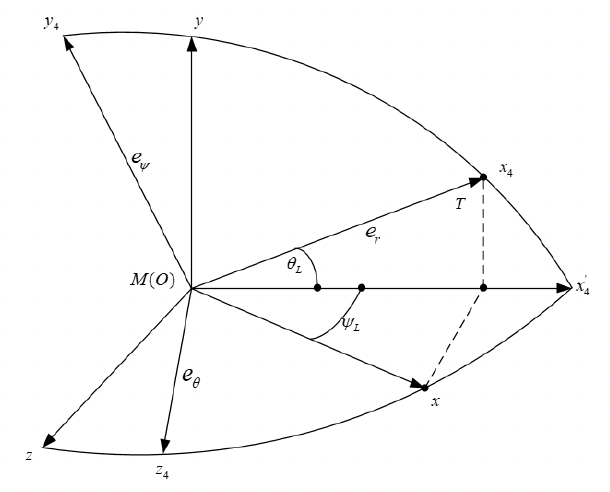
\includegraphics[width=\textwidth]{I1.png}};
  \end{tikzpicture}
  \caption{Missile and Target Dynamics}
  \label{fig:annotated_image}
\end{figure}



Based on the transformation relationship between the line-of-sight (LOS) coordinate system and the ground coordinate system, we obtain:

\[
\Omega_L = 
\begin{bmatrix}
\Omega_{x_4} \\
\Omega_{y_4} \\
\Omega_{z_4}
\end{bmatrix}
=
\begin{bmatrix}
\omega_r \\
\omega_\psi \\
\omega_\theta
\end{bmatrix}
=
\begin{bmatrix}
\dot{\psi}_L \sin \theta_L \\
\dot{\psi}_L \cos \theta_L \\
\dot{\theta}_L
\end{bmatrix}
\tag{1-24}
\]

\[
r_L =
\begin{bmatrix}
r_r \\
r_\psi \\
r_\theta
\end{bmatrix}
=
\begin{bmatrix}
r \\
0 \\
0
\end{bmatrix}
\tag{1-25}
\]

Based on equation (1-22), the relative kinematic equations of the missile and target in the LOS coordinate system can be derived:

\[
V_L =
\begin{bmatrix}
V_r \\
V_\psi \\
V_\theta
\end{bmatrix}
=
\begin{bmatrix}
\dot{r} \\
r \omega_\theta \\
-r \omega_\psi
\end{bmatrix}
\tag{1-26}
\]

Based on equation (1-23), the relative dynamic equations of the missile and target in the LOS coordinate system can be derived:

\[
\begin{cases}
\ddot{r} - r \dot{\theta}_L^2 - r \dot{\psi}_L^2 \cos^2 \theta_L = a_{T,r} - a_{M,r} \\
-r \dot{\psi}_L \cos \theta_L - 2 \dot{r} \dot{\psi}_L \cos \theta_L + 2 r \dot{\theta}_L \dot{\psi}_L \sin \theta_L = a_{T,\psi} - a_{M,\psi} \\
r \ddot{\theta}_L + 2 \dot{r} \dot{\theta}_L + r \dot{\psi}_L^2 \sin \theta_L \cos \theta_L = a_{T,\theta} - a_{M,\theta}
\end{cases}
\tag{1-27}
\]

Substituting equations (1-24) and (1-26) into (1-27), the relative dynamic equations are simplified to:


The relative dynamic equations in the line-of-sight (LOS) coordinate system are given by:

\[
\begin{cases}
\dot{V}_r = \frac{1}{r} \left( V_w^2 + V_\theta^2 \right) + a_{T,r} - a_{M,r} \\
\dot{V}_w = -\frac{V_w V_r}{r} - \frac{V_\theta^2}{r} \tan \theta_L + a_{T,w} - a_{M,w} \\
\dot{V}_\theta = -\frac{V_\theta V_r}{r} + \frac{V_w V_\theta}{r} \tan \theta_L + a_{T,\theta} - a_{M,\theta}
\end{cases}
\tag{1-28}
\]

Here:
- \( r \) and \( \dot{r} \) represent the relative distance and its derivative, respectively.
- \( V_i, V_j, a_{T,i}, a_{M,i} \) (where \( i = r, w, \theta \)) represent the relative velocity, its rate of change, and the acceleration of the target (subscript \( T \)) and the missile (subscript \( M \)) projected onto the three axes of the LOS coordinate system.


\newpage
\subsection{Formula}

In the ground coordinate system, we can derive the formulas for the relative distance and relative velocity between the missile and the target:

\[
\begin{cases} 
x_r = x_T - x_M \\ 
y_r = y_T - y_M \\ 
z_r = z_T - z_M 
\end{cases}
\tag{1-29}
\]

\[
\begin{cases} 
V_x = V_{Tx} - V_{Mx} \\ 
V_y = V_{Ty} - V_{My} \\ 
V_z = V_{Tz} - V_{Mz} 
\end{cases}
\tag{1-30}
\]

The relative distance \( r \) between the missile and the target can be expressed as:

\[
r = \sqrt{x_r^2 + y_r^2 + z_r^2}
\tag{1-31}
\]

The expressions for the line-of-sight (LOS) angle and the LOS angular rate are:

\[
\theta_L = \arctan \frac{y_r}{\sqrt{x_r^2 + z_r^2}}
\tag{1-32}
\]

\[
\psi_L = 
\begin{cases} 
-\arctan \frac{z_r}{x_r} & x_r > 0 \\ 
\pi - \arctan \frac{z_r}{x_r} & x_r < 0, z_r < 0 \\ 
-\pi - \arctan \frac{z_r}{x_r} & x_r < 0, z_r > 0 
\end{cases}
\tag{1-33}
\]

\[
\dot{\theta}_L = \frac{(x_r^2 + z_r^2)V_y - y_r(x_rV_x + z_rV_z)}{(x_r^2 + y_r^2 + z_r^2)\sqrt{x_r^2 + z_r^2}}
\tag{1-34}
\]

\[
\dot{\psi}_L = \frac{z_rV_x - x_rV_z}{x_r^2 + z_r^2}
\tag{1-35}
\]

To achieve a direct collision, it is necessary to maintain \( V_r < 0 \). Additionally, the following equations must be satisfied:
\[
\lim_{t \to t_f} V_w = 0, \quad \lim_{t \to t_f} V_\theta = 0
\tag{1-36}
\]

The missile's guidance system generates command signals through the normal accelerations \( a^c_{M,\psi} \) and \( a^c_{M,\theta} \). However, these are normal accelerations in the line-of-sight (LOS) coordinate system. Since our guidance laws are typically designed in the LOS coordinate system, but the trajectory is calculated in the ballistic coordinate system, it is necessary to transform these accelerations into the ballistic coordinate system for trajectory integration using the following matrix:
\[
\begin{bmatrix}
a^c_{Mx} \\
a^c_{My} \\
a^c_{Mz}
\end{bmatrix}
= R(\theta, \psi_v) R^T(\theta_L, \psi_L)
\begin{bmatrix}
0 \\
a^c_{M,\psi} \\
a^c_{M,\theta}
\end{bmatrix}
\tag{1-37}
\]

Here, the matrix \( R(x, y) \) is defined as:
\[
R(x, y) =
\begin{bmatrix}
\cos x \cos y & \sin x & -\cos x \sin y \\
-\sin x \cos y & \cos x & \sin x \sin y \\
\sin y & 0 & \cos y
\end{bmatrix}
\tag{1-38}
\]

The spatial True Proportional Navigation (TPN) guidance command expressions are as follows:
\[
\begin{cases}
a^c_{Mx} = 0 \\
a^c_{My} = N|r| \omega_\theta = -NV_r \dot{\theta}_L \\
a^c_{Mz} = -N|r| \omega_\psi = NV_r \dot{\psi}_L \cos \theta_L
\end{cases}
\tag{1-39}
\]

In these equations, \( N \) is the effective navigation ratio, also known as the guidance law coefficient, which satisfies the proportional navigation trajectory convergence condition: \( N > 2 \). Typically, \( N \) is set to 4.




\newpage



\section{Simulation Results}


\subsection{General approach}


Based on the three-dimensional proportional navigation guidance law mathematical model established in the previous chapter, and according to the requirements of the missile interception mission and the flight characteristics of the missile and target, the following structural block diagram is established. This diagram is used to complete the trajectory simulation of the missile interception system.

As shown in Figure 2-1, the working principle of the 3DOF guidance control loop is as follows: The seeker first calculates the relative position and relative velocity between the missile and the target based on their motion information at the current time. Then, using the formulas for calculating the relative motion information, the line-of-sight (LOS) angle and LOS angular rate are obtained. Next, guidance calculations are performed to derive the two accelerations in the LOS normal direction based on the spatial True Proportional Navigation (TPN) guidance commands. These accelerations are then transformed into the ballistic coordinate system and applied to the missile body as two accelerations in the velocity normal direction. Trajectory integration is then performed to obtain the position and velocity of the missile and target at the next time step. The measurement components are responsible for measuring the missile's motion information and feeding it back to the seeker. The relative position and velocity are obtained by taking the difference between the missile's and target's motion information. The guidance control system then repeats the above process starting from the seeker until the missile hits the target.

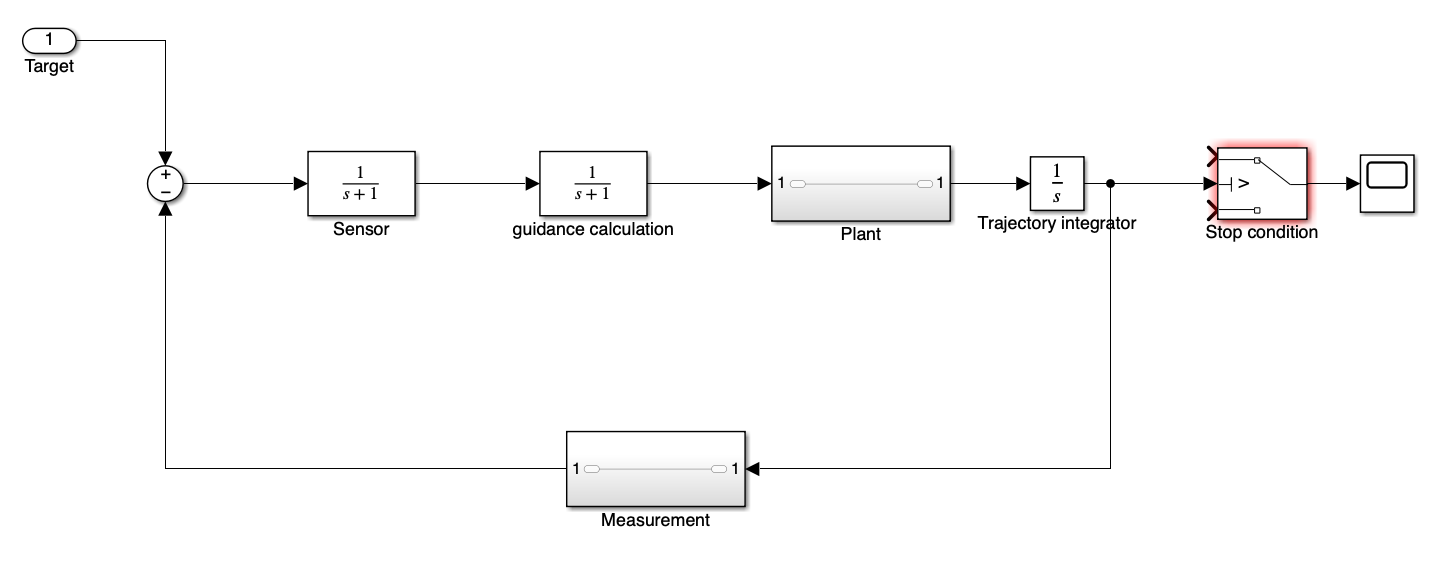
\includegraphics[width=\textwidth]{Idea.png}

\newpage

\subsection{simulation approach}
\begin{table}[h!]
  \centering
  \caption{Initial Conditions for the Missile and Target}
  \label{tab:initial_conditions}
  \begin{tabular}{|c|c|c|}
  \hline
  Parameter & Missile & Target \\
  \hline
  Initial Velocity & \(1000 \, \text{m/s}\) & \(500 \, \text{m/s}\) \\
  Trajectory pitch Angle & \(0.82 \, \text{rad}\) & \(0.0845 \, \text{rad}\) \\
  Trajectory yaw Angle & \(0.06 \, \text{rad}\) & \(0 \, \text{rad}\) \\
  \(X\) Coordinate & \(0 \, \text{m}\) & \(4000 \, \text{m}\) \\
  \(Y\) Coordinate & \(0 \, \text{m}\) & \(3000 \, \text{m}\) \\
  \(Z\) Coordinate & \(0 \, \text{m}\) & \(200 \, \text{m}\) \\
  \hline
  \end{tabular}
  \end{table}

  step size: 0.01s

  proportional navigation trajectory
  convergence condition: \( N = 4 \)

  gravitational acceleration: \( 9.81 \, \text{m/s}^2 \)

\newpage


\cite{cite-key}
\bibliographystyle{plainnat} % or another style (plain, abbrv, etc.)
\bibliography{reference}  



\newpage
\section{Matlab analysis  }
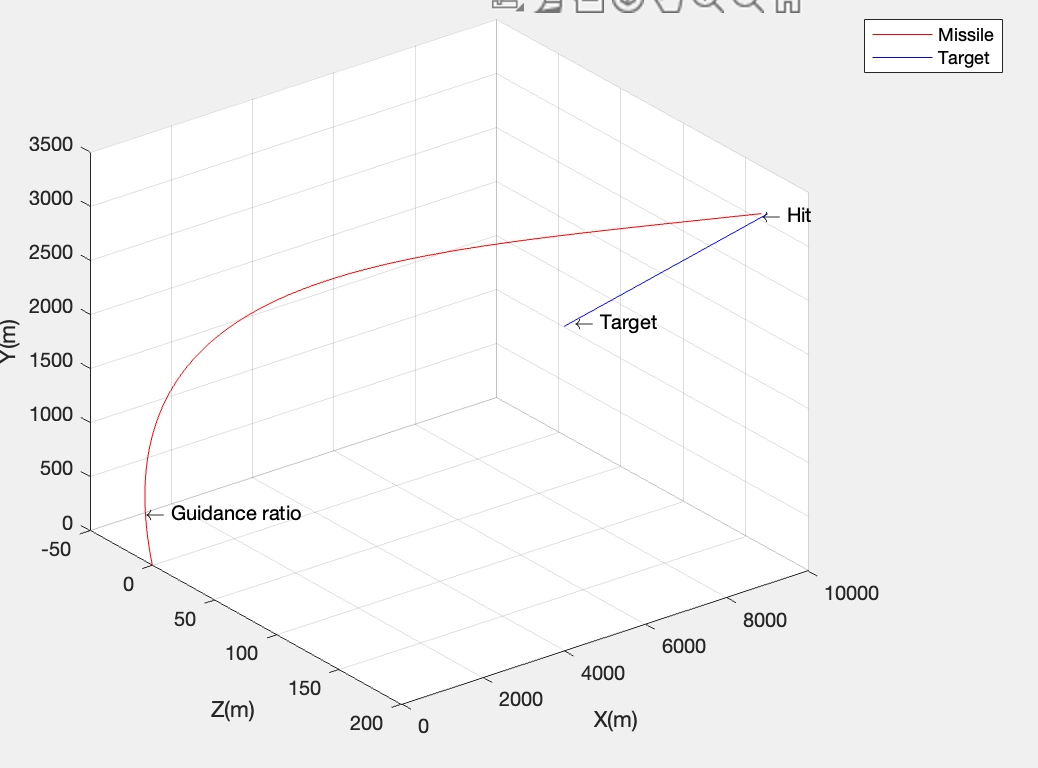
\includegraphics[width=\textwidth]{report4.png}
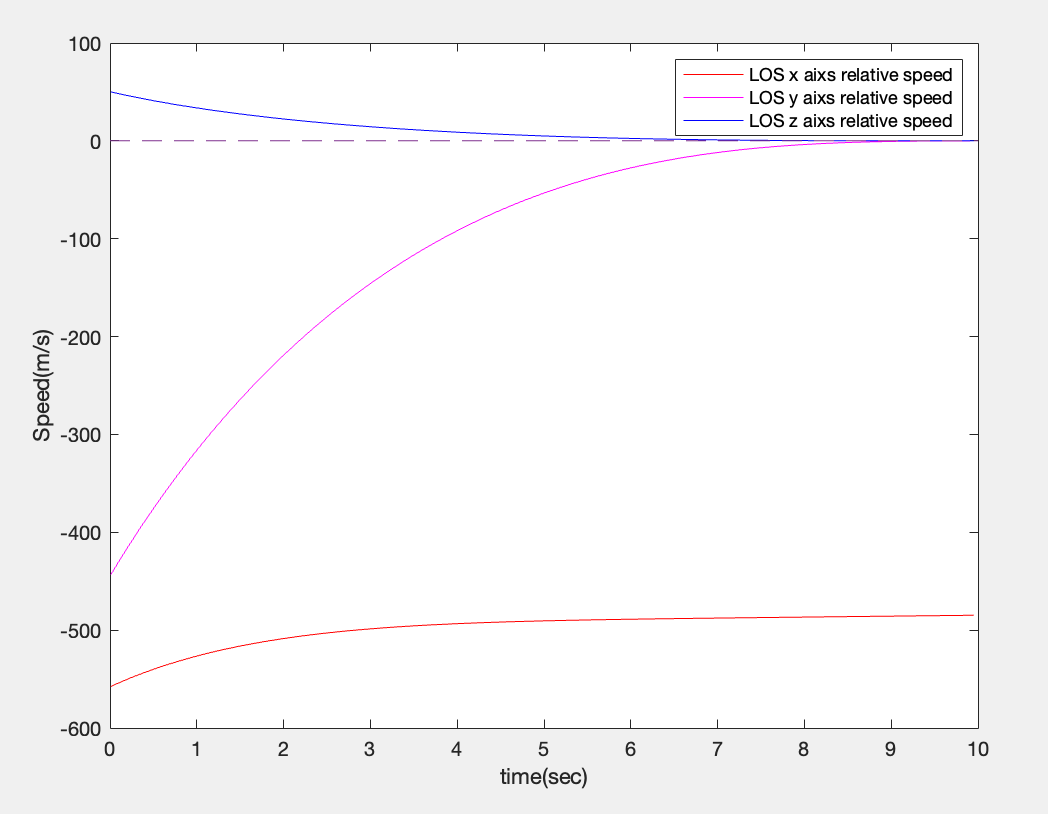
\includegraphics[width=\textwidth]{report1.png}
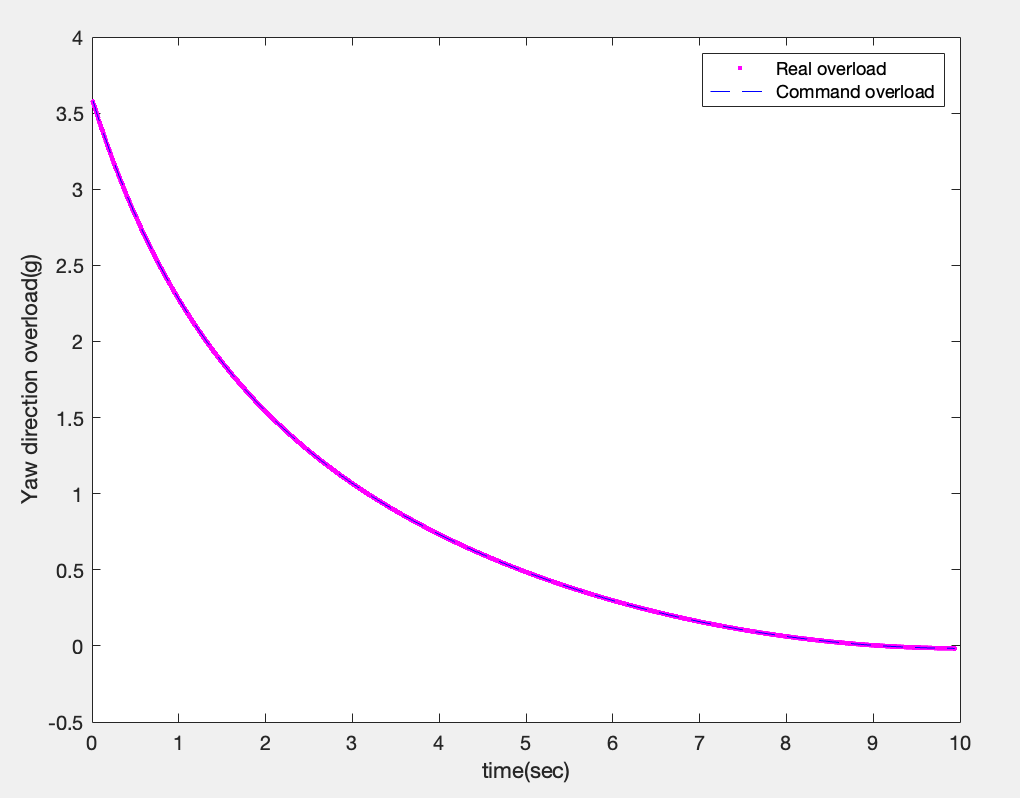
\includegraphics[width=\textwidth]{report2.png}
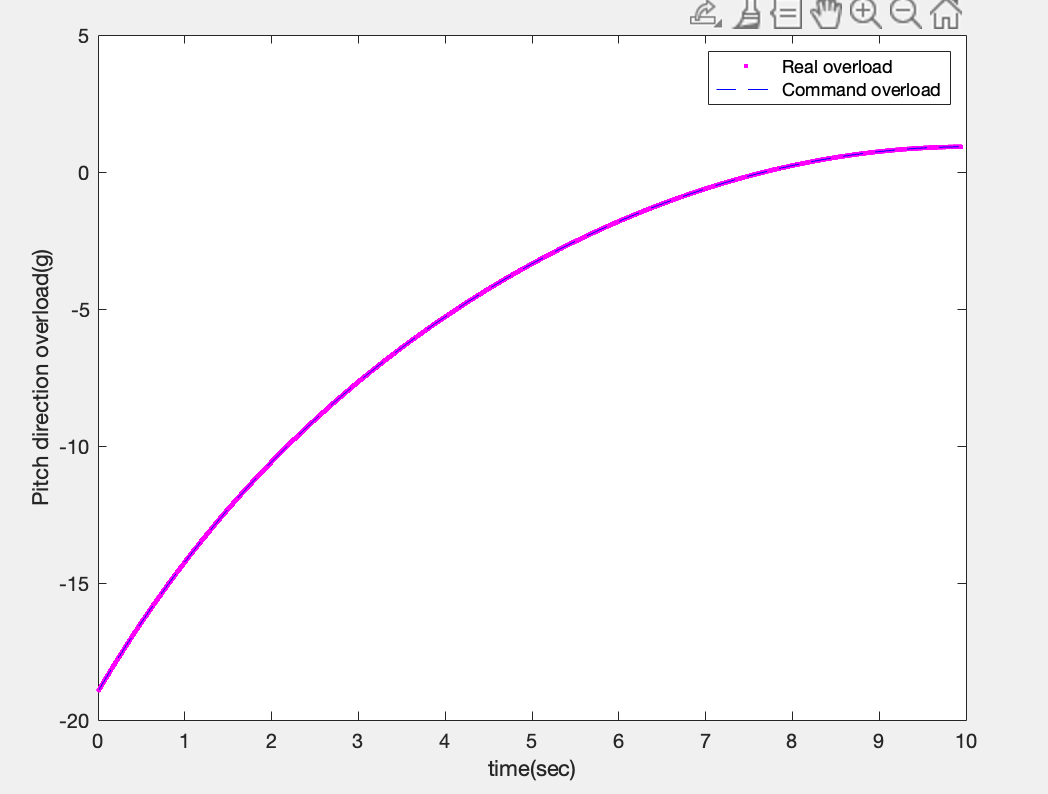
\includegraphics[width=\textwidth]{report3.png}
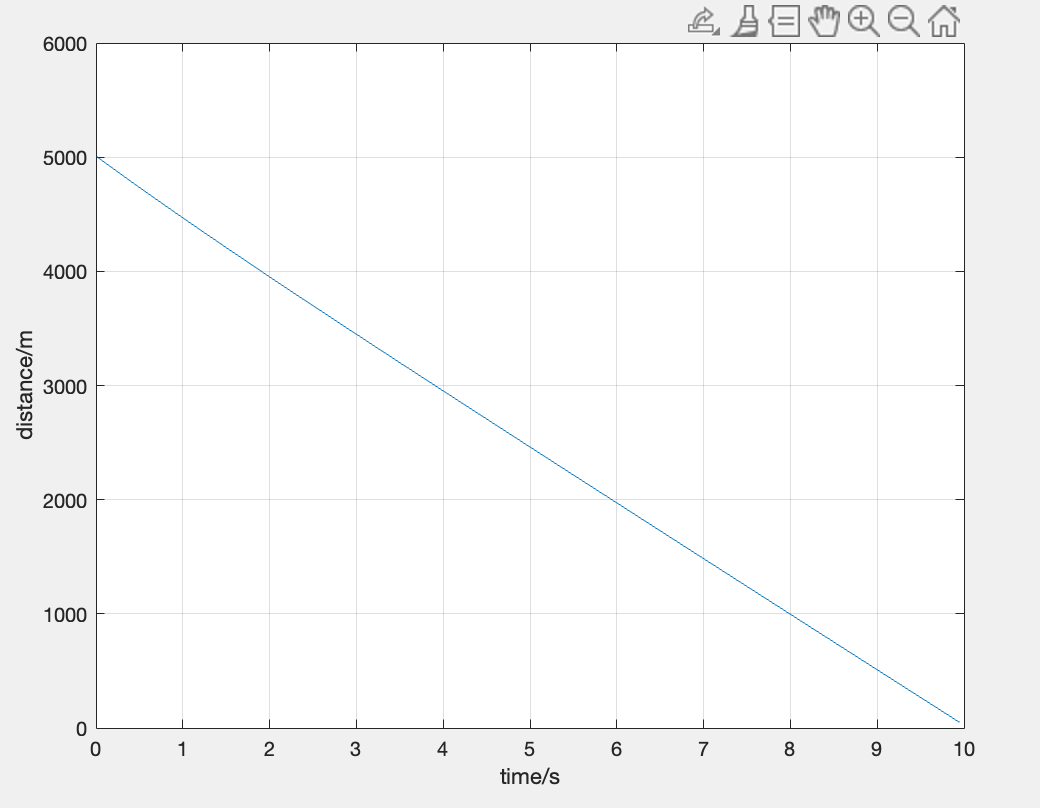
\includegraphics[width=\textwidth]{report5.png}
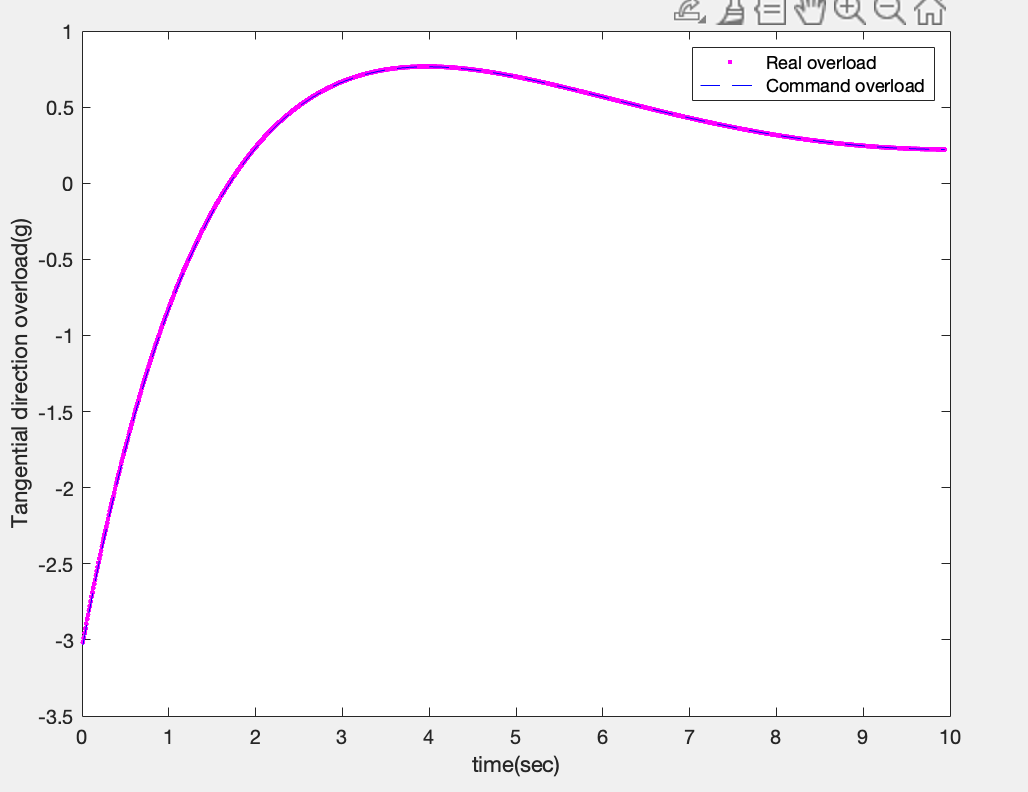
\includegraphics[width=\textwidth]{report6.png}


\end{document}